\chapter{Resultados}

Este capítulo presenta los resultados obtenidos tras la implementación de la plataforma de control y adquisición de datos, el almacenamiento de información en la base de datos SQLite y el análisis de la simulación CFD. Finalmente, se exponen los valores comparativos de velocidad de flujo de aire medidos y simulados a diferentes velocidades de giro (RPM) del ventilador.

\section{Plataforma de Control y Adquisición de Datos}
\subsection{Interfaz Web de Control}
La interfaz web desarrollada permitió a los usuarios configurar en tiempo real la velocidad del ventilador, seleccionar los sensores a monitorear y observar la evolución de las variables medidas. Como se muestra en la Figura \ref{fig:ui_plataforma}, la pantalla principal incluyó:
\begin{itemize}
    \item Un \textbf{panel de control de velocidad}, donde el operador ajustó manualmente las RPM o activó modos de operación predefinidos.
    \item Un \textbf{panel de visualización en tiempo real}, con gráficas actualizadas de corriente, voltaje, temperatura, flujo de aire y vibración. Se utilizaron librerías de JavaScript para la representación dinámica de los datos.
    \item Un \textbf{menú de configuración}, que permitía definir la frecuencia de muestreo por sensor y activar/desactivar la adquisición de cada uno.
\end{itemize}

\begin{figure}[htbp]
    \centering
    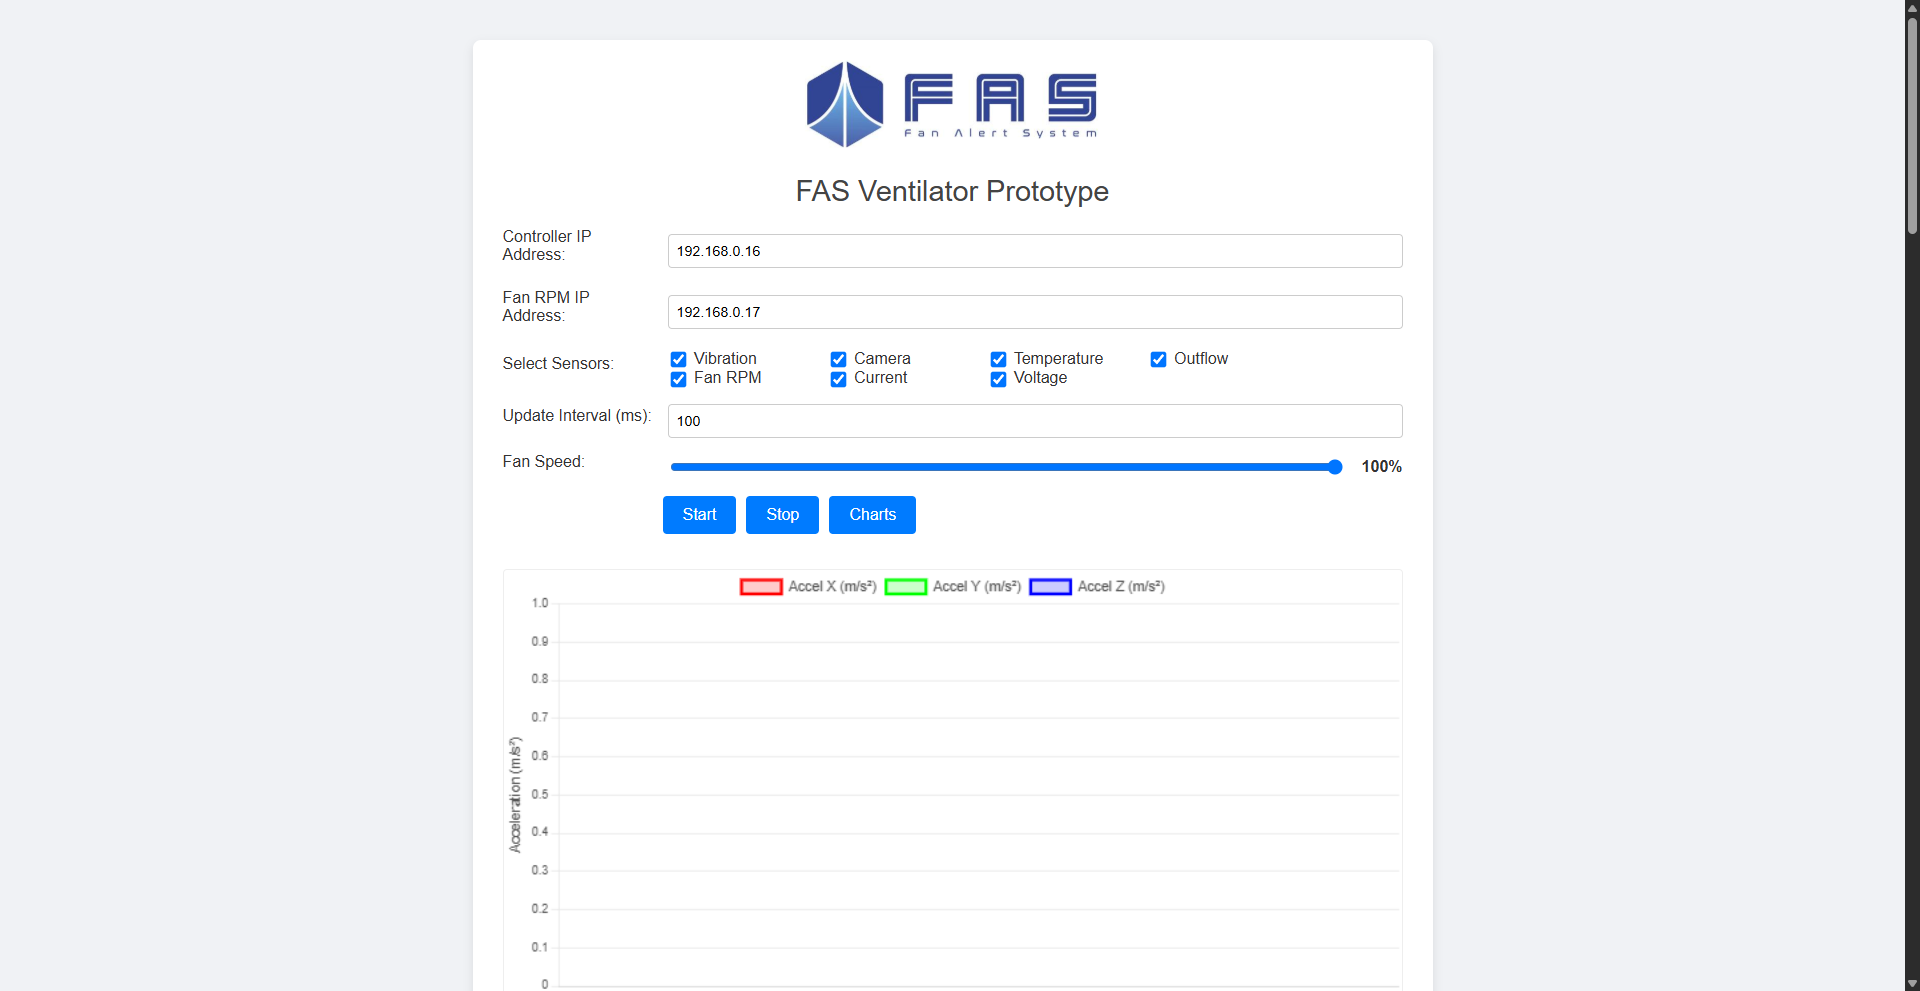
\includegraphics[width=0.75\textwidth]{images/webb.png}
    \caption{Ejemplo ilustrativo de la interfaz web de control y visualización.}
    \label{fig:ui_plataforma}
\end{figure}

\subsection{Configuración de Pruebas}
Para los ensayos de validación, se seleccionaron tres puntos de operación del ventilador: 833 RPM, 2500 RPM y 4200 RPM. En cada caso, el sistema registró continuamente las mediciones de los sensores, almacenándolas con sus marcas de tiempo. La interfaz mostró en tiempo real la evolución de las variables, lo que permitió ajustar la estrategia de medición si se detectaban anomalías o inestabilidades.

\section{Almacenamiento en Base de Datos SQLite}
\subsection{Estructura y Persistencia de Datos}
El sistema de adquisición envió los datos al servicio REST API, que posteriormente realizó la inserción de registros en la base de datos SQLite. La Tabla \ref{tab:tabla_measurements} describe la estructura principal utilizada para guardar las mediciones.

\begin{table}[htbp]
    \centering
    \caption{Estructura simplificada de la tabla \texttt{measurements} en SQLite.}
    \label{tab:tabla_measurements}
    \begin{tabular}{l l l}
    \toprule
    \textbf{Campo} & \textbf{Tipo de dato} & \textbf{Descripción}\\
    \midrule
    id & INTEGER & Clave primaria autoincremental \\
    timestamp & DATETIME & Marca de tiempo de la medición \\
    sensor\_type & TEXT & Tipo de sensor (p.ej., \textit{current}, \textit{temperature}) \\
    value & REAL & Valor medido \\
    \bottomrule
    \end{tabular}
\end{table}

Durante cada prueba, se registraron en promedio entre 400 y 600 muestras por minuto, dependiendo de la frecuencia de muestreo definida. Este volumen de datos permitió contar con información suficiente para un análisis estadístico representativo, a la vez que la ligereza de SQLite resultó adecuada para un prototipo de laboratorio.

\subsection{Consulta y Exportación de Información}
La interfaz web proporcionó consultas con filtros de fecha, tipo de sensor y rango de valores. Asimismo, en las sesiones de validación se generaron exportaciones automáticas en formato CSV, que luego sirvieron para procesar la información en hojas de cálculo o software estadístico. De este modo, se facilitó la comparación directa con los resultados numéricos de la simulación.

\newpage
\section{Resultados de la Simulación CFD}
\subsection{Configuración del Modelo Computacional}
La geometría del túnel se importó a ANSYS, donde se creó una malla combinada (hex-dominante en las regiones de flujo principal y tetraedros en cavidades complejas). Para cada simulación se asignó un número de RPM al ventilador (833, 2500 o 4200 RPM) a través de una zona de rotación (\textit{rotating domain}). Las condiciones de contorno principales fueron:
\begin{itemize}
    \item \textbf{Entrada de aire}: Presión ambiente.
    \item \textbf{Salida}: Presión abierta (0 Pa de referencia).
    \item \textbf{Paredes del túnel}: Condición de no deslizamiento (\textit{no-slip}).
\end{itemize}

El modelo de turbulencia utilizado fue \texttt{k-$\epsilon$} estándar, con discretización de segundo orden para ecuaciones de momento. La convergencia se obtuvo cuando los residuos numéricos se ubicaron por debajo de $10^{-4}$ y las variables clave (velocidad media en la salida, presión estática en la región del ventilador) estabilizaron sus valores.

%%%%%%%%%%%%%%%%%%%%%%%%%%%%%%%%%%%%%%%%%%%%%%%%%%%%%%%%%%%%%%%%%%
\subsection{Cálculo y convergencia}
Se muestran los gráficos de convergencia para los casos simulados a condiciones operacionales de 833 RPM, 2500 RPM y 4200 RPM (Fig. \ref{fig:res1}-\ref{fig:res3}).

\begin{figure}[!ht]
    \centering
    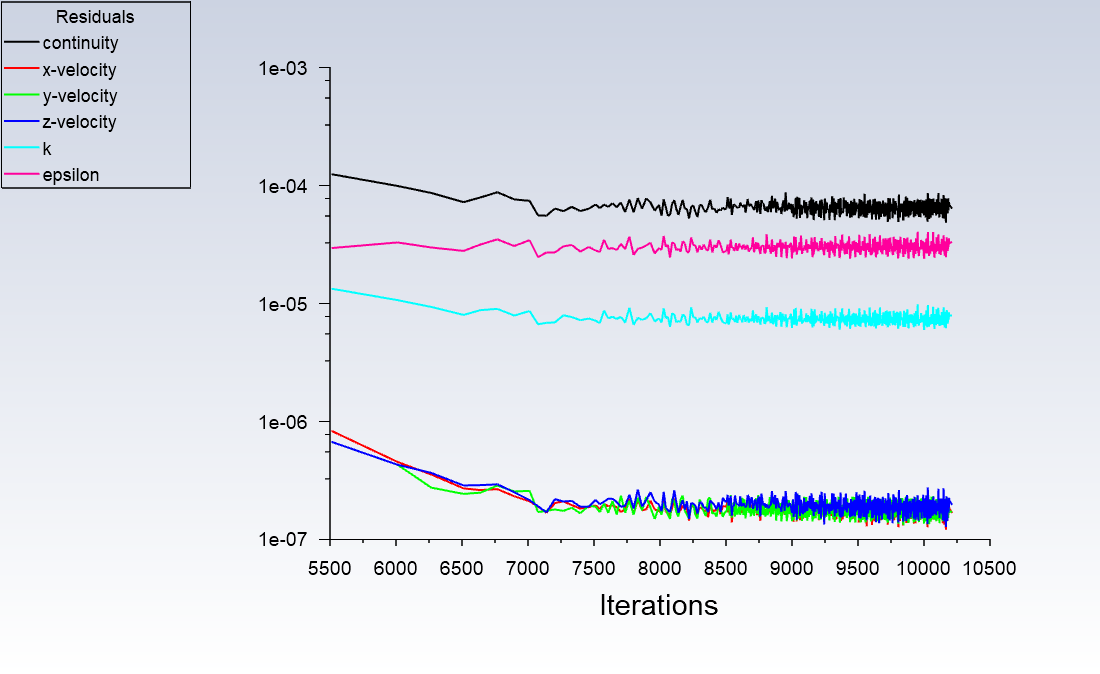
\includegraphics[width=0.7\linewidth]{images/res1.png}
    \caption{Gráfico de convergencia para 833 RPM.}
    \label{fig:res1}
\end{figure}

\pagebreak

\begin{figure}[!ht]
    \centering
    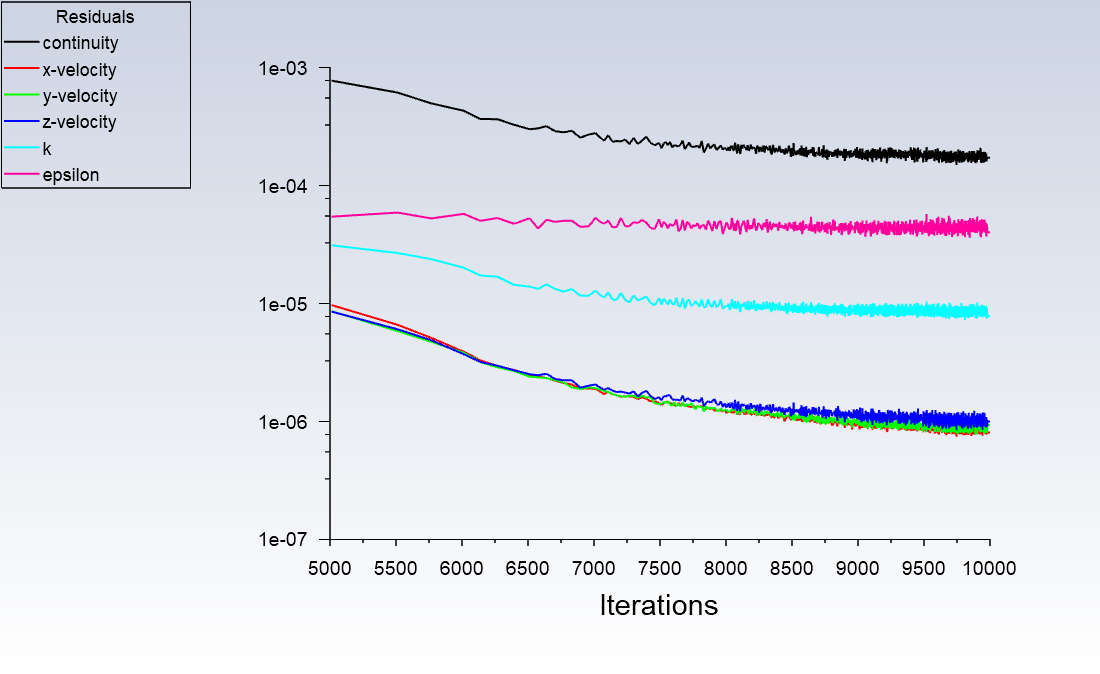
\includegraphics[width=0.7\linewidth]{images/res2.png}
    \caption{Gráfico de convergencia para 2500 RPM.}
    \label{fig:res2}
\end{figure}

\begin{figure}[!ht]
    \centering
    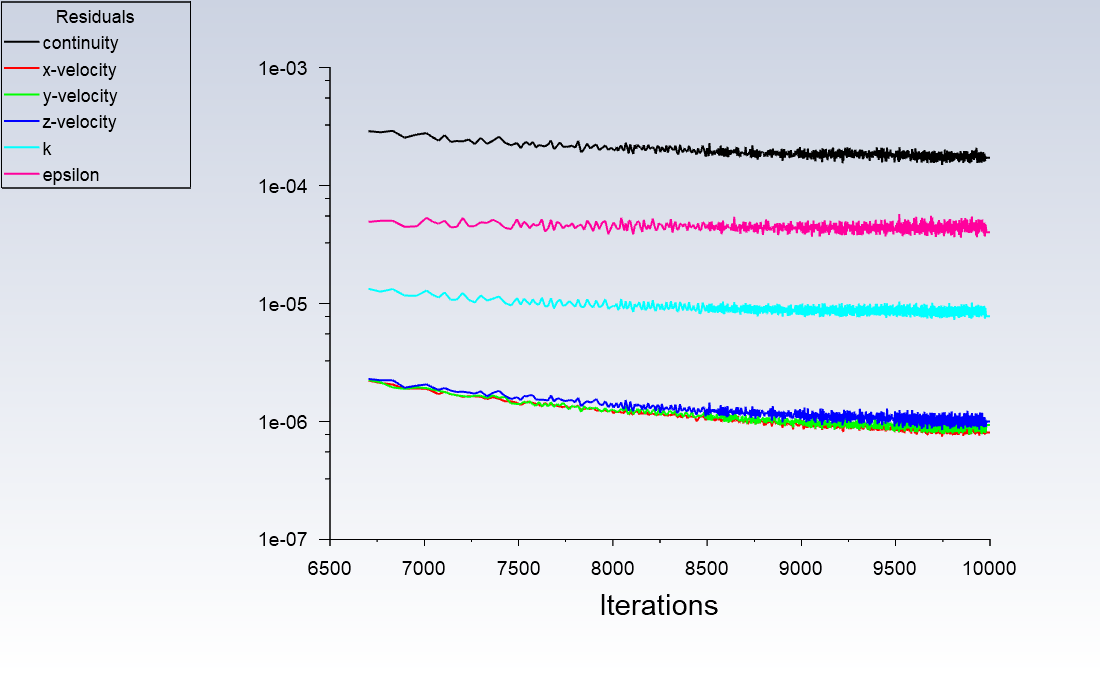
\includegraphics[width=0.7\linewidth]{images/res3.png}
    \caption{Gráfico de convergencia para 4200 RPM.}
    \label{fig:res3}
\end{figure}

Se puede notar que se alcanza la condición de convergencia en alrededor de 7000 a 9000 iteraciones.

%%%%%%%%%%%%%%%%%%%%%%%%%%%%%%%%%%%%%%%%%%%%%%%%%%%%%%%%%%%%%%%%%%%%
\newpage
\subsection{Distribución de velocidades}
La figuras \ref{fig:vel1}-\ref{fig:vel3} muestran los contornos de velocidad simulados para los casos considerados. Se aprecia que la región próxima a las aspas del ventilador presenta las mayores velocidades, que tienden a estabilizarse a medida que el flujo avanza hacia la cámara principal.

\begin{figure}[ht!]
    \centering
    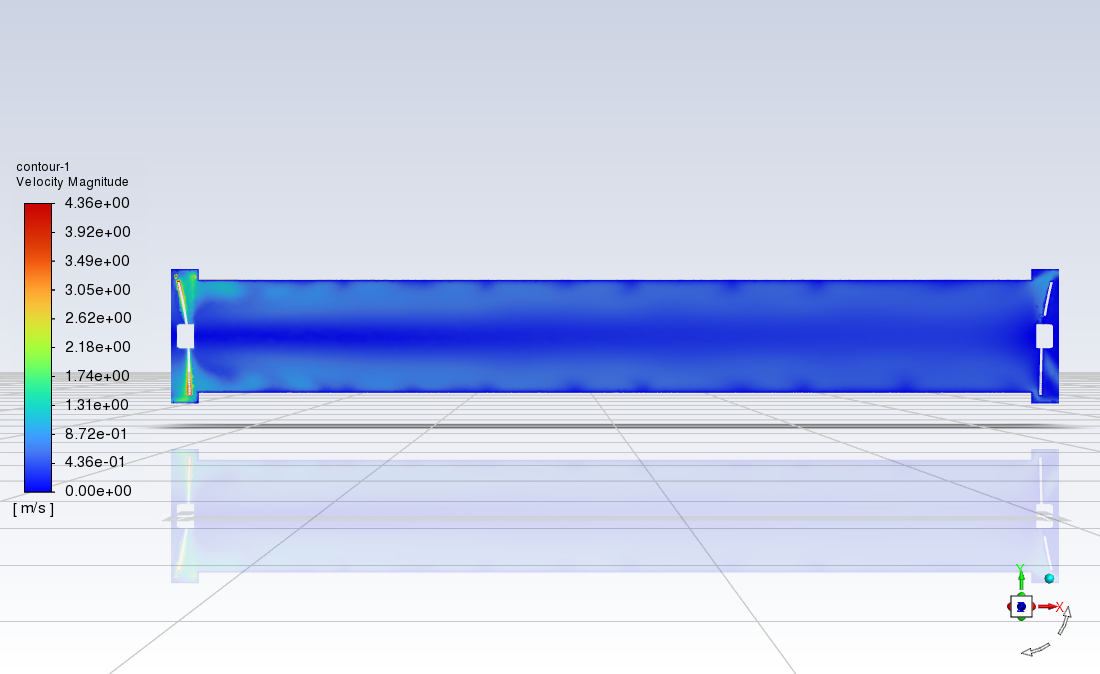
\includegraphics[width=0.9\textwidth]{images/vel1.png}
    \caption{Contornos de velocidad simulados (m/s) en el plano central del túnel para 833 RPM.}
    \label{fig:vel1}
\end{figure}

\begin{figure}[ht!]
    \centering
    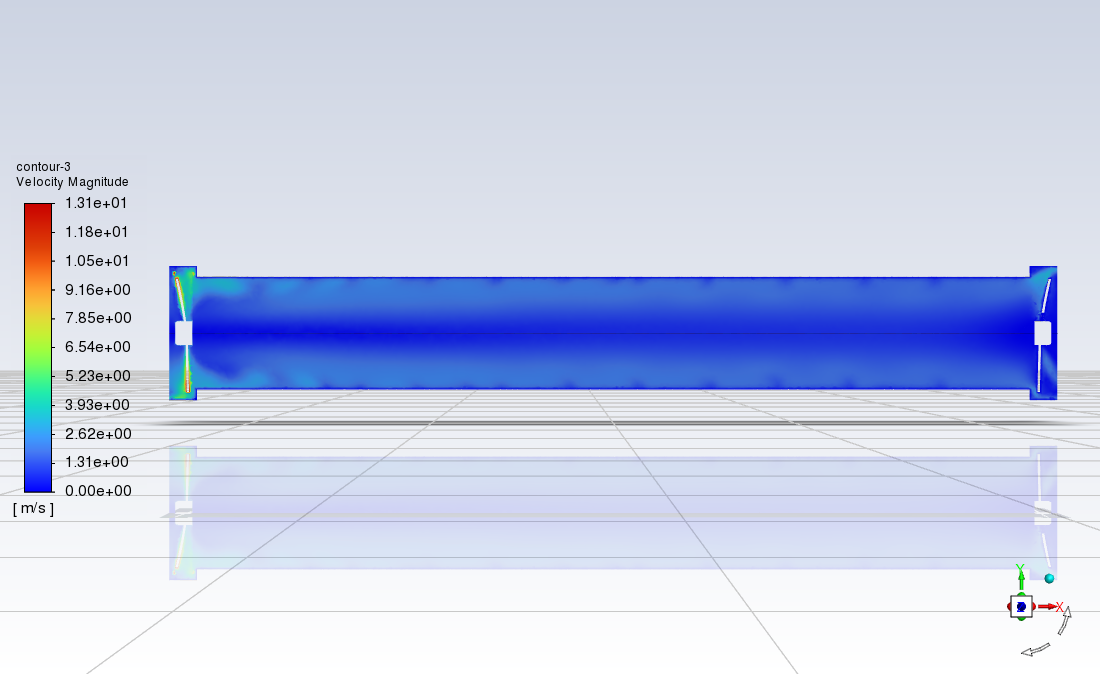
\includegraphics[width=0.9\textwidth]{images/vel2.png}
    \caption{Contornos de velocidad simulados (m/s) en el plano central del túnel para 2500 RPM.}
    \label{fig:vel2}
\end{figure}

\pagebreak

\begin{figure}[ht!]
    \centering
    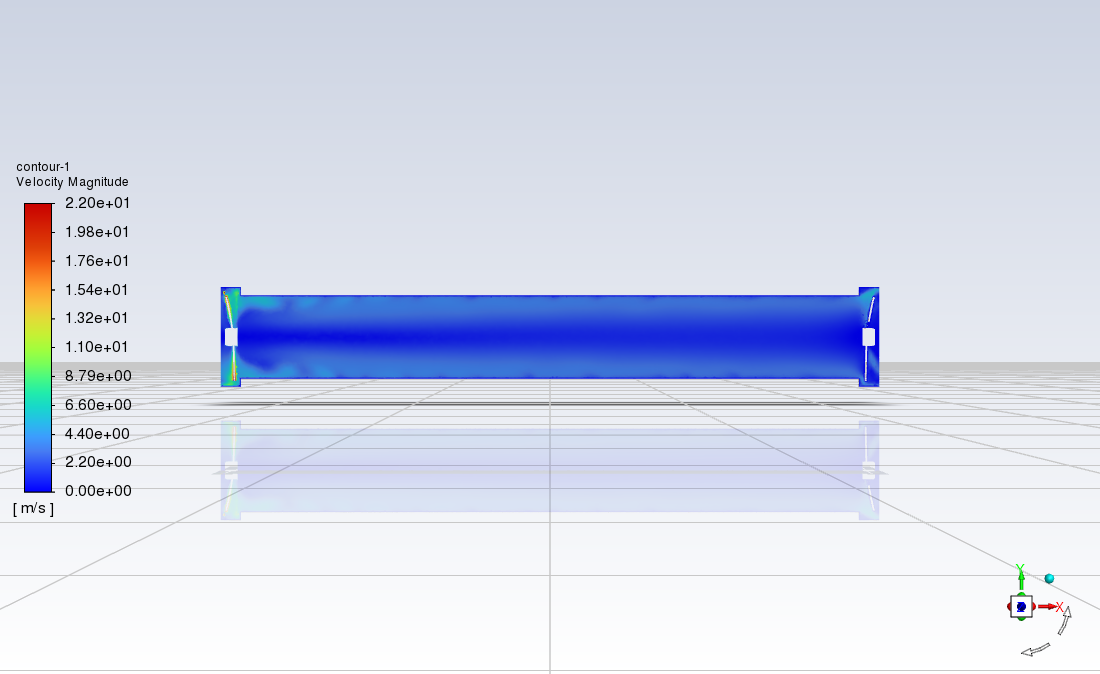
\includegraphics[width=0.9\textwidth]{images/vel3.png}
    \caption{Contornos de velocidad simulados (m/s) en el plano central del túnel para 4200 RPM.}
    \label{fig:vel3}
\end{figure}

En el plano transversal, se evidenciaron zonas de recirculación en las esquinas del conducto, especialmente a bajas RPM, lo cual concuerda con observaciones experimentales de zonas de velocidad reducida.

%%%%%%%%%%%%%%%%%%%%%%%%%%%%%%%%%%%%%%%%%%%%%%%%%%%%%%%%%%%%%%
\pagebreak
\subsection{Presiones estáticas y dinámicas}

En las figuras \ref{fig:sta1}-\ref{fig:sta3} se muestran los mapas de presión estática para los casos simulados.

\begin{figure}[!ht]
    \centering
    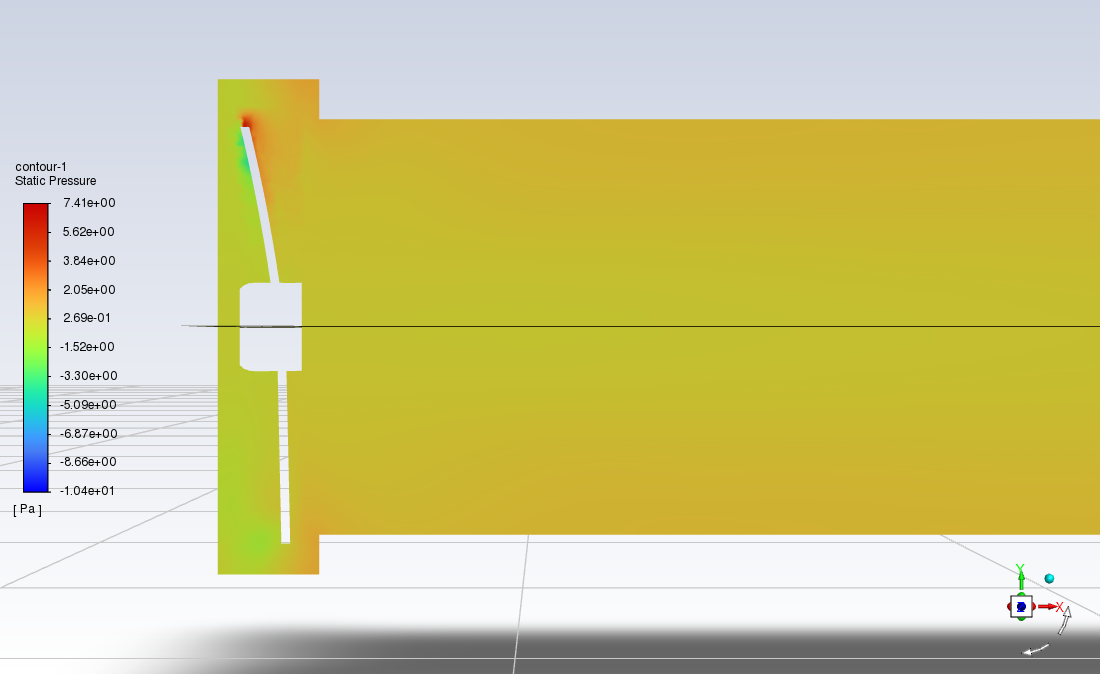
\includegraphics[width=0.6\textwidth]{images/sta1.png}
    \caption{Mapa de presión estática para 833 RPM.}
    \label{fig:sta1}
\end{figure}

\begin{figure}[!ht]
    \centering
    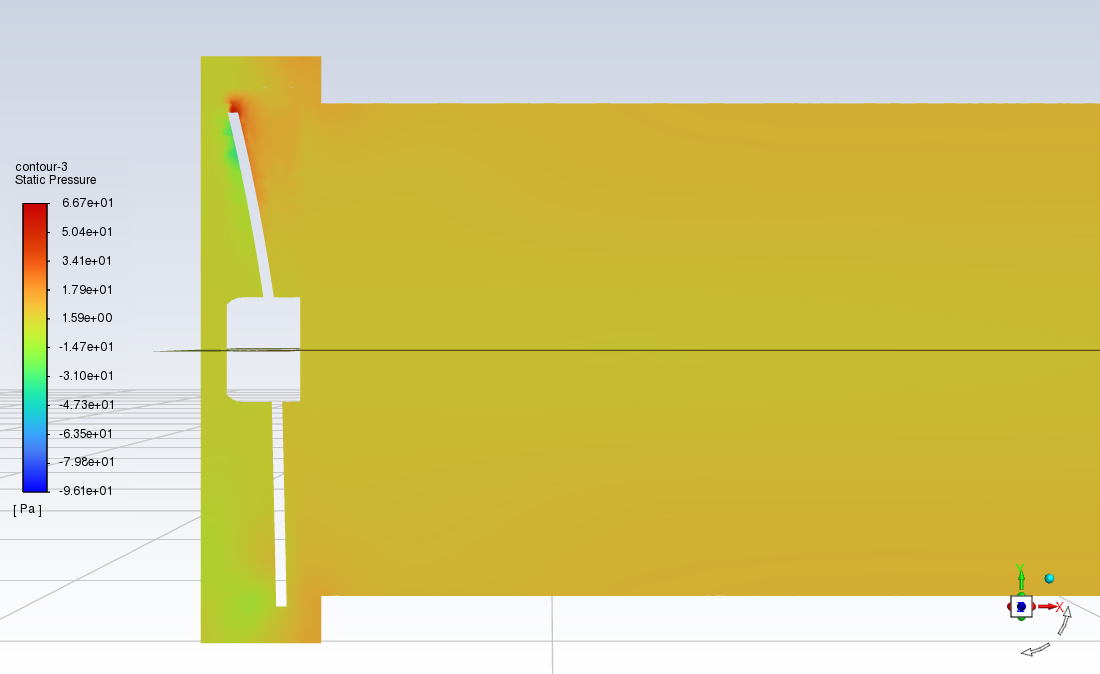
\includegraphics[width=0.6\textwidth]{images/sta2.png}
    \caption{Mapa de presión estática para 2500 RPM.}
    \label{fig:sta2}
\end{figure}

\begin{figure}[!ht]
    \centering
    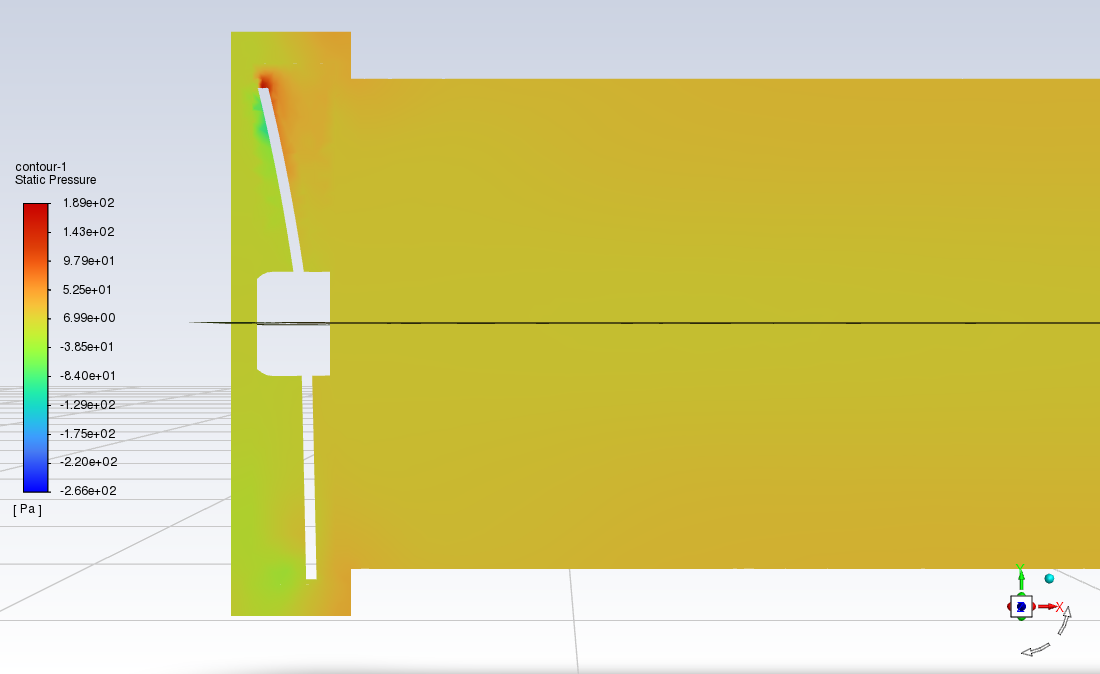
\includegraphics[width=0.6\textwidth]{images/sta3.png}
    \caption{Mapa de presión estática para 4200 RPM.}
    \label{fig:sta3}
\end{figure}

\pagebreak
En las figuras \ref{fig:dyn1}-\ref{fig:dyn3} se muestran los mapas de presión dinámica para los casos.

\begin{figure}[!ht]
    \centering
    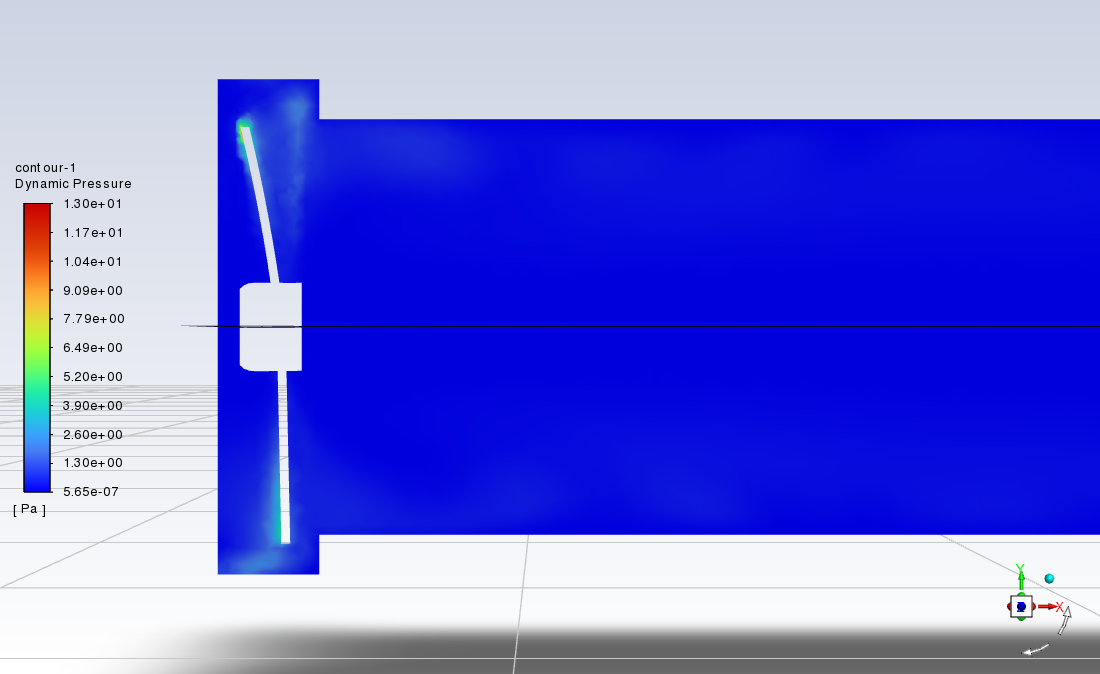
\includegraphics[width=0.6\textwidth]{images/dyn1.png}
    \caption{Mapa de presión dinámica para 833 RPM.}
    \label{fig:dyn1}
\end{figure}

\begin{figure}[!ht]
    \centering
    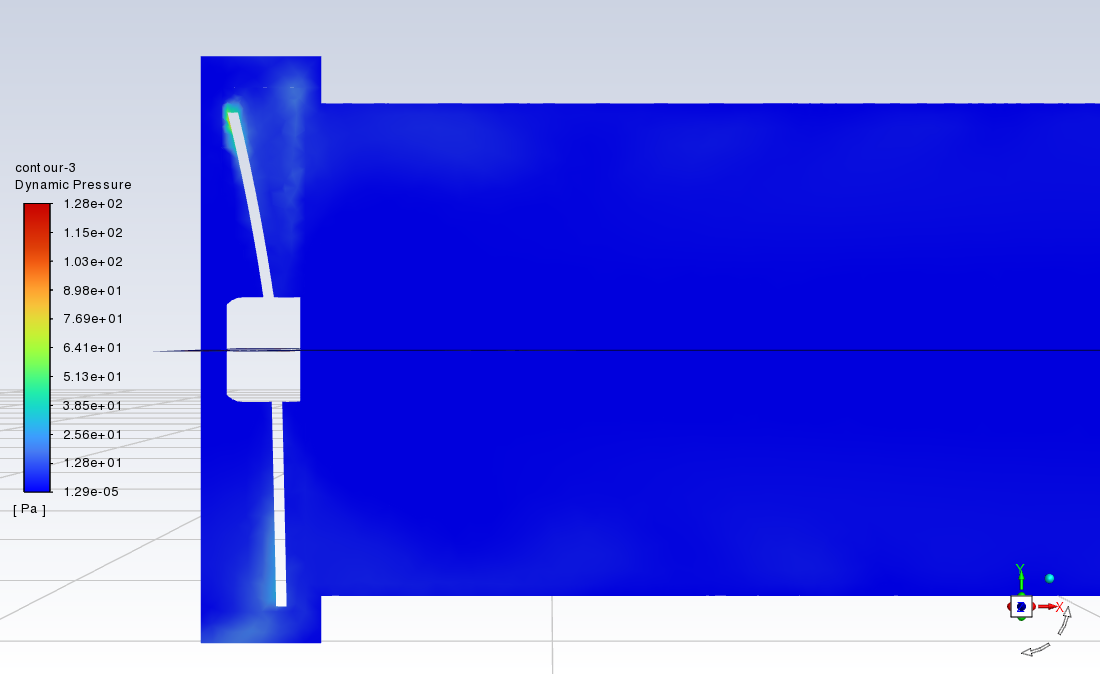
\includegraphics[width=0.6\textwidth]{images/dyn2.png}
    \caption{Mapa de presión dinámica para 2500 RPM.}
    \label{fig:dyn2}
\end{figure}

\begin{figure}[!ht]
    \centering
    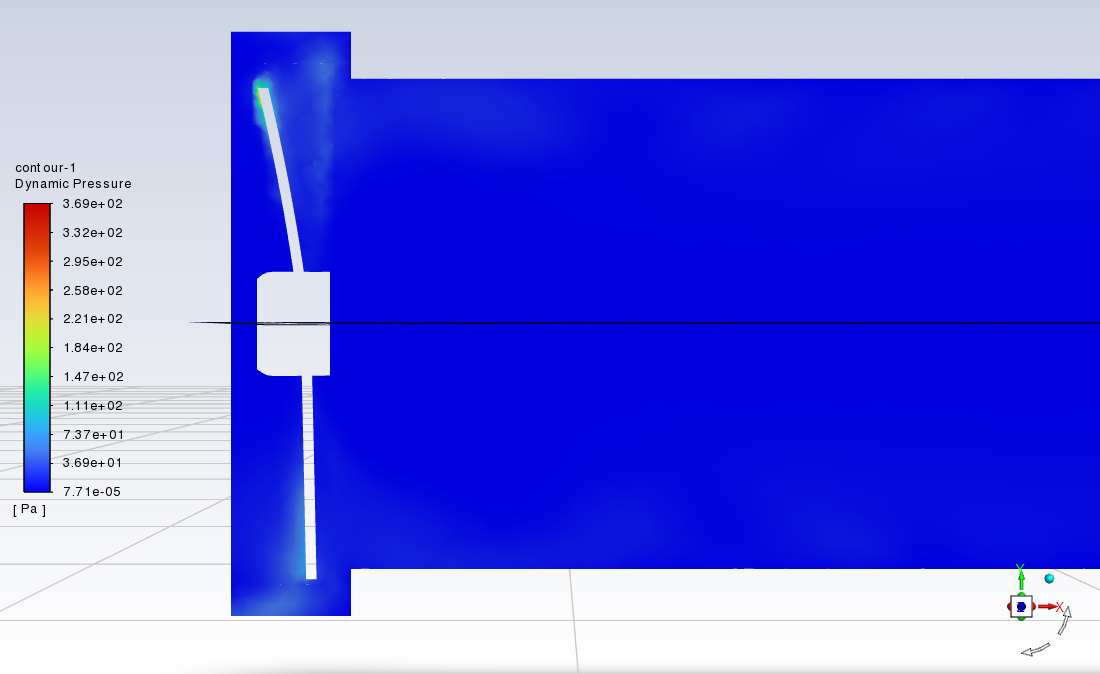
\includegraphics[width=0.6\textwidth]{images/dyn3.png}
    \caption{Mapa de presión dinámica para 4200 RPM.}
    \label{fig:dyn3}
\end{figure}

Es posible observar los mayores gradientes de presión generados en las aspas de la cámara de entrada, lo que ocasiona el flujo de entrada de viento.

%%%%%%%%%%%%%%%%%%%%%%%%%%%%%%%%%%%%%%%%%%%%%%%%%%%%%%%%%%%%%%%%%%%%%
\newpage
\subsection{Lineas de corrientes}

En las figuras \ref{fig:cor1}-\ref{fig:cor3} se presentan las lineas de corriente para los casos simulados, coloreadas según su velocidad.

\begin{figure}[ht!]
    \centering
    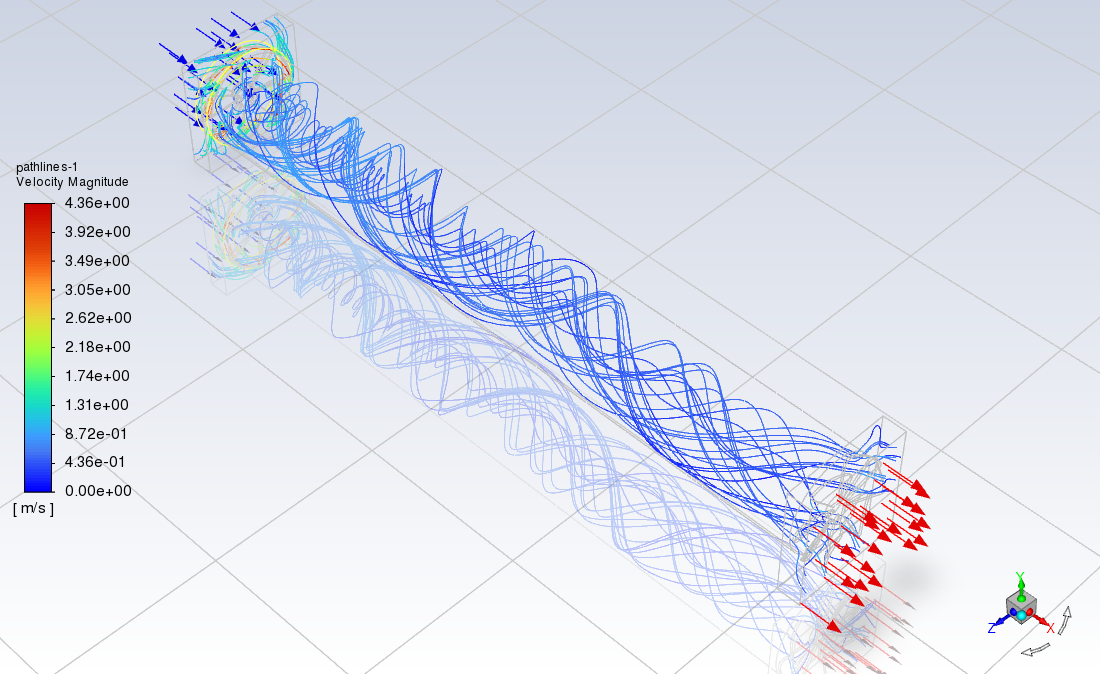
\includegraphics[width=0.9\textwidth]{images/cor1.png}
    \caption{Lineas de corriente para 833 RPM.}
    \label{fig:cor1}
\end{figure}

\begin{figure}[ht!]
    \centering
    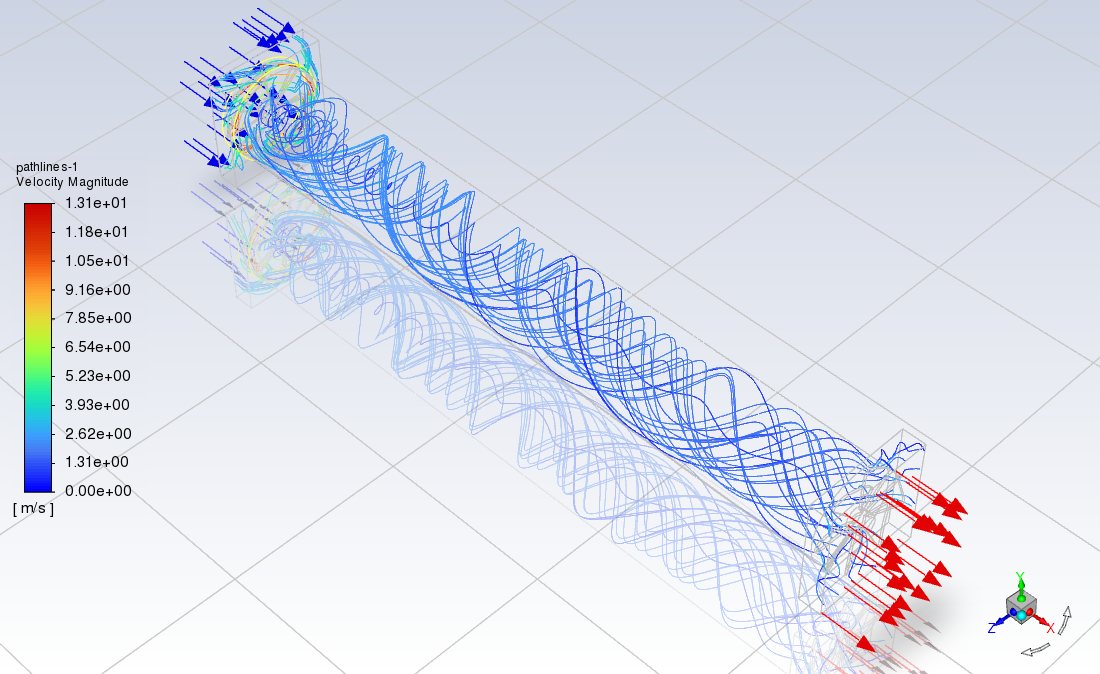
\includegraphics[width=0.9\textwidth]{images/cor2.png}
    \caption{Lineas de corriente para 2500 RPM.}
    \label{fig:cor2}
\end{figure}

\pagebreak
\begin{figure}[ht!]
    \centering
    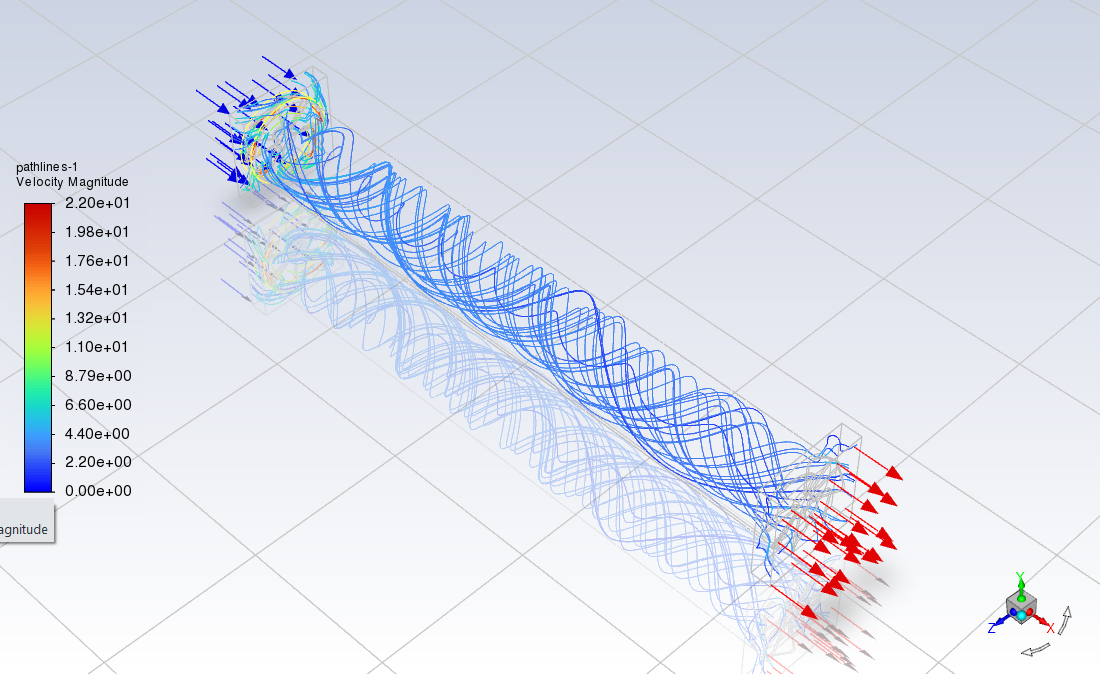
\includegraphics[width=0.9\textwidth]{images/cor3.png}
    \caption{Lineas de corriente para 4200 RPM.}
    \label{fig:cor3}
\end{figure}

Se puede notar como a mayor velocidad de rotación del ventilador incrementa la velocidad y frecuencia de remolinos en la zona perimetral del túnel.

%%%%%%%%%%%%%%%%%%%%%%%%%%%%%%%%%%%%%%%%%%%%%%%%%%%%%%%%%%%%%%%%%%%%%
\subsection{Mapas de velocidad en la cámara de salida}

Se analiza la sección transversal de la cámara de salida para extraer datos de la velocidad de flujo de viento simulado en la salida del túnel de viento para los distintos casos. En base a los datos conseguidos se realizaron promedios integrales sobre el área equivalente del instrumento de medición de velocidad del viento (diámetro de 110mm) para realizar la validación del modelo. Los mapas de velocidad de salida se muestran en las figuras \ref{fig:sal1}-\ref{fig:sal3}.

\begin{figure}[ht!]
    \centering
    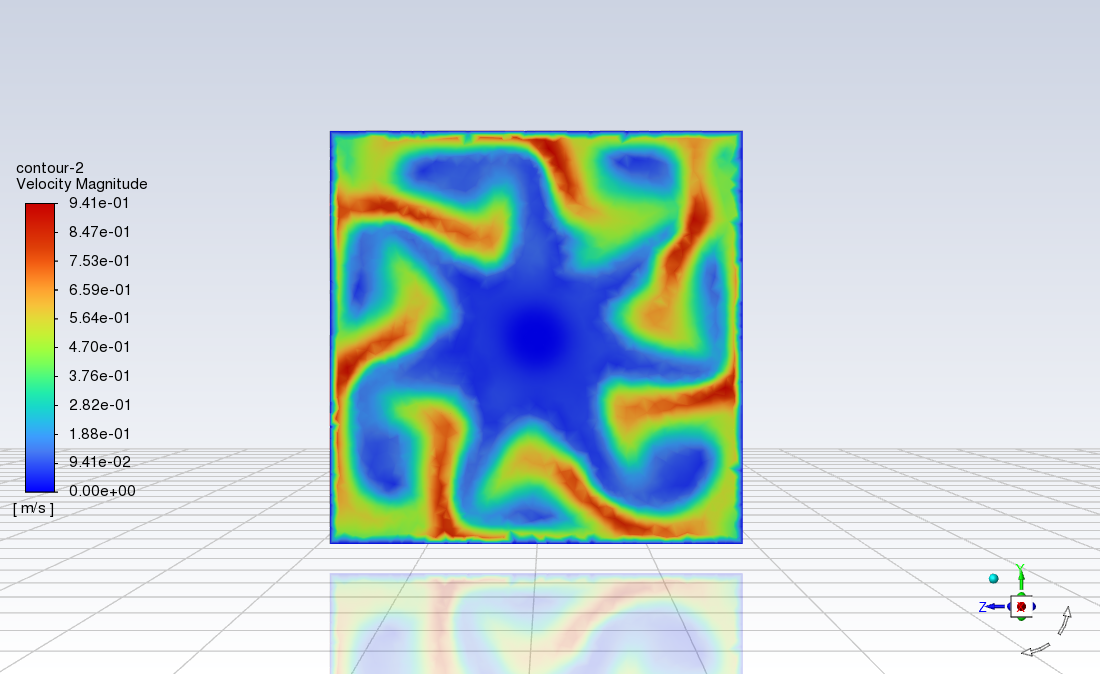
\includegraphics[width=0.6\textwidth]{images/sal1.png}
    \caption{Mapa de velocidad en la salida para 833 RPM.}
    \label{fig:sal1}
\end{figure}

\pagebreak

\begin{figure}[ht!]
    \centering
    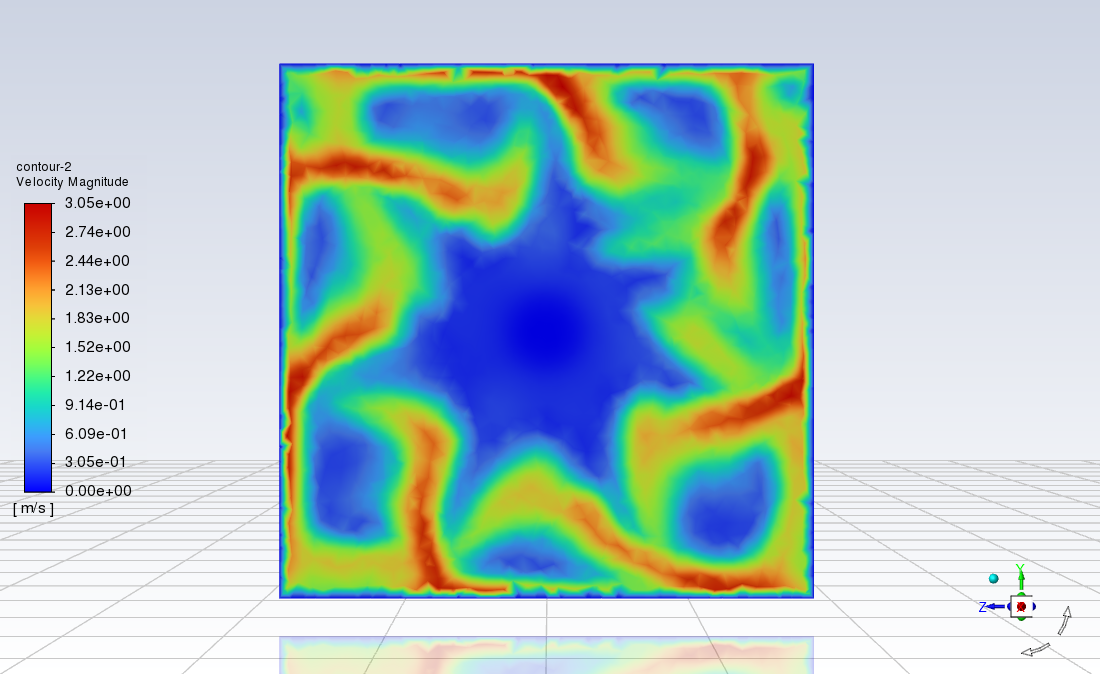
\includegraphics[width=0.6\textwidth]{images/sal2.png}
    \caption{Mapa de velocidad en la salida para 2500 RPM.}
    \label{fig:sal2}
\end{figure}

\begin{figure}[ht!]
    \centering
    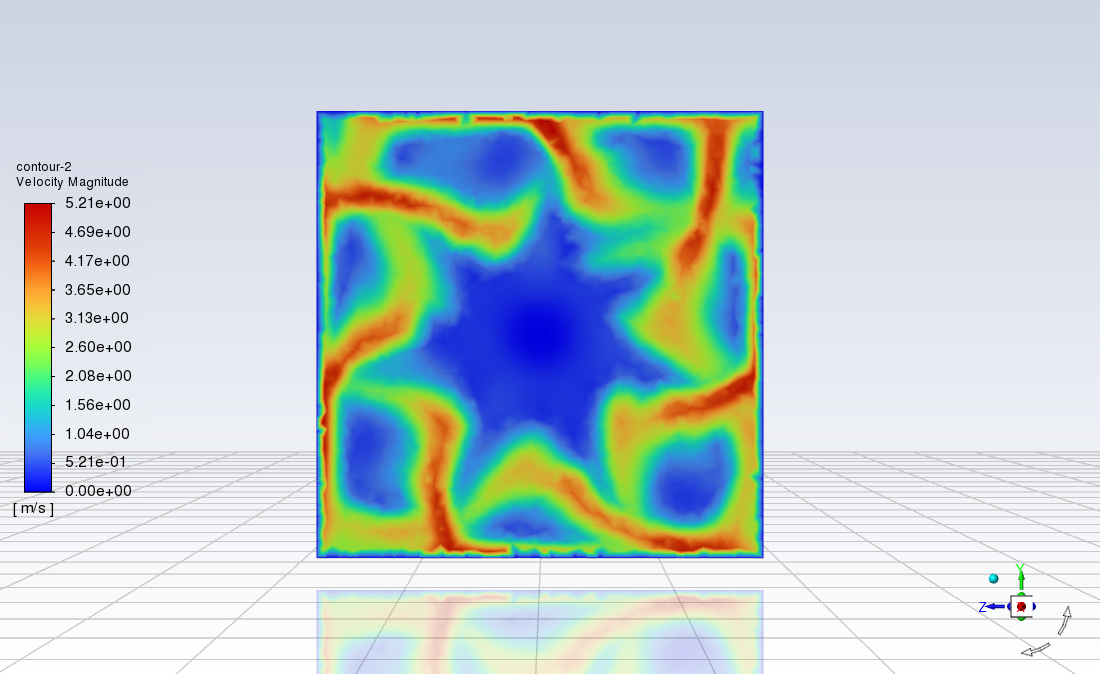
\includegraphics[width=0.6\textwidth]{images/sal3.png}
    \caption{Mapa de velocidad en la salida para 4200 RPM.}
    \label{fig:sal3}
\end{figure}

Se observa como debido a la obstrucción del anemómetro en la cámara de salida se generan zonas de alta velocidad en los alrededores de las aspas. 

%%%%%%%%%%%%%%%%%%%%%%%%%%%%%%%%%%%%%%%%%%%%%%%%%%%%%%%%%%%%%%%%%%%%%
\newpage
\section{Comparación de Velocidad de Flujo de Aire a Distintas RPM}
\subsection{Mediciones Experimentales vs. Simulación}
Para la validación cuantitativa, se midieron las velocidades promedio en la cámara principal a una distancia de aproximadamente 690 mm del ventilador, utilizando el sensor de flujo de aire indirecto y un anemómetro calibrado de 110mm de diámetro. Se utiliza una integral de área sobre la superficie correspondiente al anemómetro para determinar la velocidad. En la Tabla \ref{tab:comp_velocidades} se listan los valores medios experimentales (\(\bar{v}_{\text{exp}}\)) y los simulados (\(\bar{v}_{\text{sim}}\)), junto con el porcentaje de error relativo.

\begin{table}[htbp]
    \centering
    \caption{Comparación de velocidades promedio medidas y simuladas a diferentes RPM del ventilador.}
    \label{tab:comp_velocidades}
    \begin{tabular}{cccccc}
    \toprule
    \multirow{2}{*}{\textbf{RPM}} & \multicolumn{2}{c}{\textbf{Velocidad (m/s)}} & \multirow{2}{*}{\textbf{Error \%}} \\
    \cmidrule(r){2-3}
    & $\bar{v}_{\text{exp}}$ & $\bar{v}_{\text{sim}}$ &  \\
    \midrule
    833 & 0.63 & 0.46 & 26.98\% \\
    2500 & 1.80 & 1.34 & 25.56\% \\
    4200 & 2.75 & 2.12 & 22.91\% \\
    \bottomrule
    \end{tabular}
\end{table}

Se observó que el error porcentual promedio se ubicó cerca de 25\%, valor considerado aceptable para un prototipo a escala, dados los supuestos simplificadores (geometría idealizada y simplificada, supuestas condiciones isotérmicas y ausencia de pérdidas detalladas en el eje del ventilador).

\subsection{Análisis de Resultados}
Los resultados muestran una tendencia coherente: a medida que se incrementa la velocidad de giro del ventilador, el flujo de aire presenta mayor velocidad tanto en el experimento como en la simulación. La presencia de un error prácticamente constante sugiere que el modelo CFD capta de manera consistente la dinámica del flujo, aunque podrían afinarse ciertos aspectos (malla en la zona del impulsor o modelos de turbulencia más avanzados) para disminuir la diferencia.

\section{Resumen de los Resultados}
En conclusión, se logró:
\begin{itemize}
    \item Implementar una \textbf{plataforma de control y adquisición de datos} funcional, basada en Arduino, una REST API y un panel web, con almacenamiento ligero en SQLite.
    \item Obtener \textbf{mediciones experimentales} confiables de corriente, voltaje, temperatura, vibración y velocidad de aire en el túnel de viento a escala.
    \item Desarrollar un \textbf{modelo CFD} en ANSYS cuyos resultados de velocidad de flujo muestran concordancia satisfactoria (errores promedios del orden de 25\%) frente a los datos reales en un rango de 833 a 4200 RPM.
\end{itemize}

Estos hallazgos sientan las bases para la validación del sistema y aportan indicios de que las metodologías propuestas —tanto la plataforma de medición como el modelo de simulación— pueden escalarse a condiciones mineras reales o utilizarse como punto de partida para implementar algoritmos de mantenimiento predictivo.

%%%%%%%%%%%%%%%%%%%%%%%%%%%%%%%%%%%%%%%%%%%%%%%%%%%%%%%%%%%%%%%%%%%%
\section{Evaluación Cualitativa de Datos}

Tras aplicar la metodología descrita para la evaluación cualitativa de los datos, se obtuvieron los siguientes hallazgos principales:

\subsection{Patrones de Operación Observados}
\begin{itemize}
    \item \textbf{Rangos de RPM estables:} En la mayoría de los ensayos, se identificó un rango de revoluciones (aproximadamente entre 833 y 4200 RPM) en el cual el ventilador mantiene un comportamiento estable, con lecturas de corriente y vibraciones relativamente constantes.
    \item \textbf{Regiones de posible sobrefuerzo:} No fue posible detectar zonas de sobreesfuerzo. El comportamiento fue nominal para todas las velocidades sin mayores variaciones en temperatura.
\end{itemize}

\subsection{Comparación Cualitativa entre Datos Experimentales y Simulación}
\begin{itemize}
    \item \textbf{Similitud en la distribución de velocidades:} Las mediciones reales de la velocidad del viento (mediante el anemómetro) mostraron valores de magnitud coherentes con los obtenidos en la simulación CFD, especialmente en el rango medio de velocidades.
    \item \textbf{Impacto de vibraciones y pérdidas:} El prototipo experimental presentó vibraciones adicionales que no se capturaron en la simulación, lo que sugiere que, para mejorar la concordancia, habría que refinar el modelado mecánico y acoplarlo a los fenómenos fluidodinámicos.
\end{itemize}

\subsection{Relaciones entre Variables Clave}
\begin{itemize}
    \item \textbf{RPM--Vibraciones:} Se constató que, en general, un incremento progresivo de RPM se asocia con mayores valores de vibración.
    \item \textbf{RPM--Velocidad del Viento:} Existió una correlación directa y estable en la mayor parte de los ensayos.
    \item \textbf{Corriente--Temperatura:} Al aumentar la carga eléctrica, no fue posible registrar grandes cambios de temperatura, lo que sugiere que el ventilador opera en su rango nominal y no se está sobreesforzando.
\end{itemize}

\subsection{Posible Viabilidad de un Modelo Predictivo}
\begin{itemize}
    \item \textbf{Variedad de datos:} La existencia de mediciones tanto en condiciones normales como en regímenes de sobreesfuerzo sugiere que los conjuntos de datos cuentan con cierto grado de diversidad. Esto resulta prometedor para futuros enfoques predictivos.
    \item \textbf{Inconsistencias menores:} Aunque se detectaron disparidades en escenarios de alta RPM, la mayor parte de la información muestra coherencia interna suficiente como para servir de base a un análisis más profundo y a la eventual creación de un modelo de mantenimiento predictivo.
    \item \textbf{Posibles Variables Complementarias:} La incorporación de más señales (por ejemplo, análisis de espectros de vibración o monitoreo del desgaste físico en el tiempo) podría incrementar la confianza y robustez de un futuro modelo.
\end{itemize}

\noindent
En términos generales, la evaluación cualitativa muestra que los datos disponibles describen de forma razonable el comportamiento del ventilador a diferentes regímenes de operación. Existe una relación consistente entre las variables clave (RPM, velocidad de viento, vibraciones), lo cual se considera indicio de que sería factible avanzar hacia modelos más sofisticados de predicción y mantenimiento si se profundiza
